\documentclass[11pt,letterpaper]{article}
\usepackage[lmargin=1in,rmargin=1in,bmargin=1in,tmargin=1in]{geometry}
\usepackage{checkins}

\pgfplotsset{soldot/.style={color=black,only marks,mark=*},
		holdot/.style={color=black,fill=white,only marks,mark=*},
		compat=1.12
}

\newcommand{\boxseven}[4]{%
	\draw[thick] (0,0) -- (4,0) -- (4,4) -- (0,4) -- (0,0);
	\draw[thick] (0,2) -- (4,2);
	\draw[thick] (2,0) -- (2,4);
	% '7'
	\draw[line width=0.03cm] (1.7,2.2) -- (2.3,2.2) -- (1.7,1.6);
	% Entries
	\node at (1,3) {$#1$};	% u
	\node at (3,1) {$#2$};	% dv
	\node at (1,1) {$#3$};	% du
	\node at (3,3) {$#4$};	% 
}

\usetikzlibrary{calc}
\usepackage{booktabs}
\tikzset{Arrow Style/.style={text=black, font=\boldmath}}
\newcommand{\tikzmark}[1]{%
    \tikz[overlay, remember picture, baseline] \node (#1) {};%
}
\newcommand*{\XShift}{0.5em}
\newcommand*{\YShift}{0.5ex}
\NewDocumentCommand{\DrawArrow}{s O{} m m m}{%
    \begin{tikzpicture}[overlay,remember picture]
        \draw[->, thick, Arrow Style, #2] 
                ($(#3.west)+(\XShift,\YShift)$) -- 
                ($(#4.east)+(-\XShift,\YShift)$)
        node [midway,above] {#5};
    \end{tikzpicture}%
}

% -------------------
% Content
% -------------------
\begin{document}
\thispagestyle{title}

% 08/21
\checkin{08/21} The integral $\ds\int x \sqrt[3]{x - 2} \;dx$ can be treated as a `shifting integral' by using the $u$-substitution $u= x - 2$. \pspace

\sol The statement is \textit{true}. We `want' to be able to distribute the $x$ across the cube-root but we cannot---this is not a valid operation. However, if we make the $u$-substitution $u= x - 2$, then we will be able to distribute in a way that makes this integral `routine.' So, let $u= x - 2$, then $du= dx$. Moreover, because $u= x - 2$, we know that $x= u + 2$. But then\dots
	\[
	\int x \sqrt[3]{x - 2} \;dx= \int (u + 2) \sqrt[3]{u} \;du= \int \left( u^{4/3} + 2 u^{1/3} \right) \;du= \tfrac{3}{7}\, u^{7/3} + \tfrac{3}{4} \cdot 2u^{4/3} + C= \tfrac{3}{7} (x - 2)^{7/3} + \tfrac{3}{2} (x - 2)^{4/3} + C
	\]
Note that a computer algebra system may write the answer (though you will \textit{not} be expected to) like this:
	\[
	\tfrac{3}{7} (x - 2)^{7/3} + \tfrac{3}{2} (x - 2)^{4/3} + C= (x - 2)^{4/3} \left( \tfrac{3}{7} (x - 2) + \tfrac{3}{2} \right) + C= (x - 2)^{4/3} \left( \tfrac{3}{7}x + \tfrac{9}{14} \right) + C= \tfrac{3}{14} (x - 2)^{4/3} \left( 2x + 3 \right) + C
	\] \pvspace{1.3cm}



% 08/26
\checkin{08/26} Using integration-by-parts to evaluate $\ds\int x \tan^{-1}(x) \;dx$, one chooses $u= \tan^{-1} x$ and $dv= x$. \pspace

\sol The statement is \textit{true}. Using LIATE, the first term that appears is `I' for inverse trig. Therefore, we choose $u= \tan^{-1} x$. But then $dv= x$. We then fill in our box:
	\[
	\begin{tikzpicture}
	\boxseven{\tan^{-1} x}{x}{\dfrac{1}{1 + x^2}}{\dfrac{x^2}{2}}
	\end{tikzpicture}
	\]
Using the `rule of 7', we have\dots
	\[
	\int x \tan^{-1} x \;dx= \dfrac{1}{2}\, x^2 \tan^{-1} x - \dfrac{1}{2} \int \dfrac{x^2}{1 + x^2} \;dx
	\]
We now need only evaluate the integral on the right. Dividing $1 + x^2$ into $x^2$, we have a remainder of $-1$, i.e. $\dfrac{x^2}{1 + x^2}= 1 + \dfrac{-1}{1 + x^2}$. Therefore, we have\dots
	\[
	\dfrac{1}{2} \int \dfrac{x^2}{1 + x^2} \;dx= \dfrac{1}{2} \int \left( 1 + \dfrac{-1}{1 + x^2} \right) \;dx= \dfrac{1}{2} \left( x - \tan^{-1} x \right) + C
	\]
But then\dots
	\[
	\begin{aligned}
	\int x \tan^{-1} x \;dx&= \dfrac{1}{2}\, x^2 \tan^{-1} x - \dfrac{1}{2} \int \dfrac{x^2}{1 + x^2} \;dx \\[0.3cm]
	&= \dfrac{1}{2}\, x^2 \tan^{-1} x - \dfrac{1}{2} \left( x - \tan^{-1} x \right) + C  \\[0.3cm]
	&= \dfrac{1}{2}\, x^2 \tan^{-1} x - \dfrac{1}{2} \, x + \dfrac{1}{2}\, \tan^{-1} x + C \\[0.3cm]
	&= \dfrac{x^2 \tan^{-1} x - x + \tan^{-1} x}{2} + C \\[0.3cm]
	&= \dfrac{(x^2 + 1) \tan^{-1} x - x}{2} + C
	\end{aligned}
	\] \pvspace{1.3cm}



% 08/28
\checkin{08/28} The integral $\ds\int e^x \sin(3x) \;dx$ can be treated as an integration-by-parts `looping' integral. \pspace

\sol The statement is \textit{true}. Using integration-by-parts for $\ds\int e^x \sin(3x) \;dx$ would result in an integral that would `loop' back to itself. Generally, an integrand of the form $\text{exponential} \cdot (\text{sin or cos})$ or $\text{trig} \cdot \text{trig}$ will have this property. Using traditional integration-by-parts, by LIATE, we choose $u= \sin(3x)$ and $dv= e^x$. Filling out our box, we have\dots
	\[
	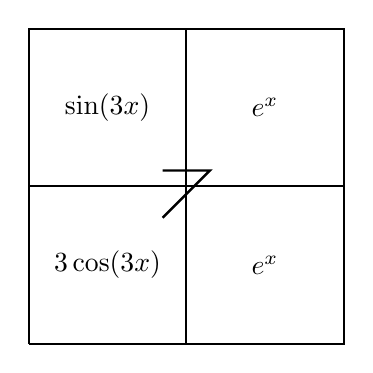
\begin{tikzpicture}
	\boxseven{\sin(3x)}{e^x}{3 \cos(3x)}{e^x}
	\end{tikzpicture}
	\]
Using the `rule of seven', we then have\dots
	\[
	\int e^x \sin(3x) \;dx= e^x \sin(3x) - \int 3e^x \cos(3x) \;dx
	\]
To integrate $\ds\int 3e^x \cos(3x) \;dx$, we again use integration-by-parts. Using LIATE, we choose $u= 3 \cos(3x)$ and $dv= e^x$. Filling out the box, we have\dots
	\[
	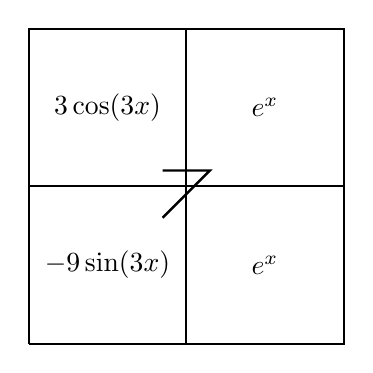
\begin{tikzpicture}
	\boxseven{3\cos(3x)}{e^x}{-9\sin(3x)}{e^x}
	\end{tikzpicture}
	\]
Using the `rule of seven', we then have 
	\[
	\int 3e^x \cos(3x) \;dx= 3 e^x \cos(3x) - \int -9e^x \sin(3x) \;dx= 3 e^x \cos(3x) + 9 \int e^x \sin(3x) \;dx
	\]
But then we have\dots
	\[
	\hspace{-1cm} \int e^x \sin(3x) \;dx= e^x \sin(3x) - \int 3e^x \cos(3x) \;dx= \int e^x \sin(3x) \;dx= e^x \sin(3x) - \left( 3 e^x \cos(3x) + 9 \int e^x \sin(3x) \;dx \right)
	\]
Therefore, we have\dots
	\[
	\begin{gathered}
	\int e^x \sin(3x) \;dx= e^x \sin(3x) - \left( 3 e^x \cos(3x) + 9 \int e^x \sin(3x) \;dx \right) \\[0.2cm]
	\int e^x \sin(3x) \;dx= e^x \sin(3x) - 3 e^x \cos(3x) - 9 \int e^x \sin(3x) \;dx \\[0.2cm]
	10 \int e^x \sin(3x) \;dx= e^x \sin(3x) - 3 e^x \cos(3x) \\[0.2cm]
	\int e^x \sin(3x) \;dx= \dfrac{e^x \sin(3x) - 3 e^x \cos(3x)}{10} + C \\[0.2cm]
	\int e^x \sin(3x) \;dx= \dfrac{e^x}{10} \,\big( \sin(3x) - 3 \cos(3x) \big) + C
	\end{gathered}
	\]
Alternatively, we can use an alteration of the tabular method of integration-by-parts. We choose $u= \sin(3x)$ and $dv= e^x$. We then have\dots
	\[
	\begin{array}{c @{\hspace*{1.3cm}} c} \toprule
	u & dv \\ \cmidrule(lr){1-2}
	\sin(3x) \tikzmark{Left 1} & \tikzmark{Right 1} e^x \\[0.5cm]
	3 \cos(3x) \tikzmark{Left 2} & \tikzmark{Right 2} e^x \\[0.3cm]
	-9 \sin(3x) \tikzmark{Left 3}  & \tikzmark{Right 3} e^x 
	
	\DrawArrow{Left 1}{Right 2}{+}
	\DrawArrow{Left 2}{Right 3}{--}
	\DrawArrow{Left 3}{Right 3}{\!\!\!\!\!$\phantom{}_{\genfrac{}{}{0pt}{}{}{+}}$}
	\end{array}
	\]
Therefore, we have\dots
	\[
	\int e^x \sin(3x) \;dx= e^x \sin(3x) - 3 \cos(3x) e^x - 9 \int e^x \sin(3x) \;dx
	\]
Solving for our integral, we have\dots
	\[
	\begin{gathered}
	\int e^x \sin(3x) \;dx= e^x \sin(3x) - 3 \cos(3x) e^x - 9 \int e^x \sin(3x) \;dx \\[0.2cm]
	10 \int e^x \sin(3x) \;dx= e^x \sin(3x) - 3 e^x \cos(3x) \\[0.2cm]
	\int e^x \sin(3x) \;dx= \dfrac{e^x \sin(3x) - 3 e^x \cos(3x)}{10} + C \\[0.2cm]
	\int e^x \sin(3x) \;dx= \dfrac{e^x}{10} \,\big( \sin(3x) - 3 \cos(3x) \big) + C
	\end{gathered}
	\] \pvspace{1.3cm}



% 09/02
\checkin{09/02} To integrate $\ds\int \cot^2 x \csc^2 x \;dx$ as a trigonometric integral, one could make the substitution $u= \cot x$. \pspace

\sol The statement is \textit{true}. If one let $u= \csc x$, we would have $du= -\csc x \cot x$. Setting aside a $\cot x$ for the $du$, this would leave only a single $\cot x$ term in the integrand---which we cannot replace with a Pythagorean identity. However, this is not an issue if we let $u= \cot x$. If $u= \cot x$, then $du= -\csc^2 x \,dx$. But then\dots
	\[
	\int \cot^2 x \csc^2 x \;dx= -\int \cot^2 x \cdot -\csc^2 x \;dx= -\int u^2 \;du= -\dfrac{u^3}{3} + C= -\dfrac{\cot^3 x}{3} + C
	\] \pvspace{1.3cm}



% 09/04
\checkin{09/04} To integrate $\ds\int \dfrac{x^2}{\sqrt{x^2 + 9}} \;dx$, one can make the substitution $x= 3 \cot \theta$. \pspace

\sol The statement is \textit{true}. Observe that the $x^2 + 9$ `resembles' a term from the Pythagorean Theorem. This suggests that a trig. substitution might be useful. Because $a^2 + b^2= c$, we see that $a^2 + b^2$ corresponds to $x^2 + 9$, i.e. $a^2$ corresponds to $x^2$ and $b^2$ corresponds to $9$. This implies that $a= x$ and $b= 3$. But then $c^2= x^2 + 9$, i.e. $c= \sqrt{x^2 + 9}$. We construct a right triangle with these legs and hypotenuse: 
	\[
	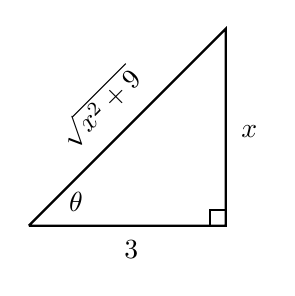
\begin{tikzpicture}
	\draw[line width=0.03cm] (0,0) -- (2.5,0) -- (2.5,2.5) -- (0,0);
	\draw[line width=0.03cm] (2.3,0) -- (2.3,0.2) -- (2.5,0.2);
	\node at (0.6,0.3) {$\theta$};
	\node at (1.3,-0.3) {$3$};
	\node at (2.8,1.2) {$x$};
	\node[rotate = 45] at (0.9,1.5) {$\sqrt{x^2 + 9}$};
	\end{tikzpicture}
	\]
But then $\tan \theta= \tfrac{x}{3}$, which implies $x= 3 \tan \theta$. While this \text{seems} like it makes the statement of the problem false, this is not the only right triangle we could have constructed. If we had instead drawn
	\[
	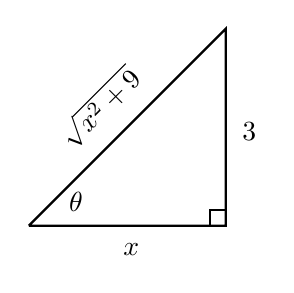
\begin{tikzpicture}
	\draw[line width=0.03cm] (0,0) -- (2.5,0) -- (2.5,2.5) -- (0,0);
	\draw[line width=0.03cm] (2.3,0) -- (2.3,0.2) -- (2.5,0.2);
	\node at (0.6,0.3) {$\theta$};
	\node at (1.3,-0.3) {$x$};
	\node at (2.8,1.2) {$3$};
	\node[rotate = 45] at (0.9,1.5) {$\sqrt{x^2 + 9}$};
	\end{tikzpicture}
	\]
We would have $\tan \theta= \tfrac{3}{x}$, which implies that $x \tan \theta= 3$, so that $x= \tfrac{3}{\tan \theta}= 3 \cot \theta$. This is the substitution in the problem statement. Both the substitutions $x= 3 \cot \theta$ and $x= 3 \tan \theta$ are viable trig. substitutions to compute this integral. \pvspace{1.3cm}



% 09/09
\checkin{09/09} The partial fraction decomposition of $\dfrac{x + 4}{x^2(x - 3)}$ has the form $\dfrac{Ax + B}{x^2} + \dfrac{C}{x - 3}$. \pspace

\sol The statement is \textit{false}. For a partial fraction decomposition, one first needs to be sure that the degree of the numerator is smaller than the degree of the denominator---which is the case here. One then needs to be sure that the denominator is factored completely---which is the case here. One then needs to `run' through each power of the factored terms of the denominator---being sure that the numerator term for quadratic factors is linear. In this case, the denominator terms are $x$ (up to power 2) and $x - 3$. Therefore, the partial fraction decomposition is\dots
	\[
	\dfrac{x + 4}{x^2(x - 3)}= \dfrac{A}{x} + \dfrac{B}{x^2} + \dfrac{C}{x - 3}
	\]
Although the term $x^2$ is quadratic, the base---$x$---is linear. Hence, its numerator terms will always be constant---never linear. This is the mistake in the decomposition given in the problem statement. \pvspace{1.3cm}
































\end{document}